\refsubsection{Concepts}{subsec:concepts}
\todo{Graphs, eg. concept maps, co-occurrence graphs}
\todo{Classical text representations, eg.tfidf
Categories of algorithms, eg. algorithms on feature vectors, kernelized - algorithms}


\refsubsection{Definitions and Notations}{subsec:definitions_and_notations}
\todo{Lay groundwork for the later description of the problem}
\todo{Introductions to used classifiers, concepts}
\todo{Concretize the problem and its notation}
\todo{Comparison of the used data sources}

\subsubsection{Classification Task}

\subsubsection{Graphs}

\paragraph{Concept Map}
\begin{figure}[h]
\centering
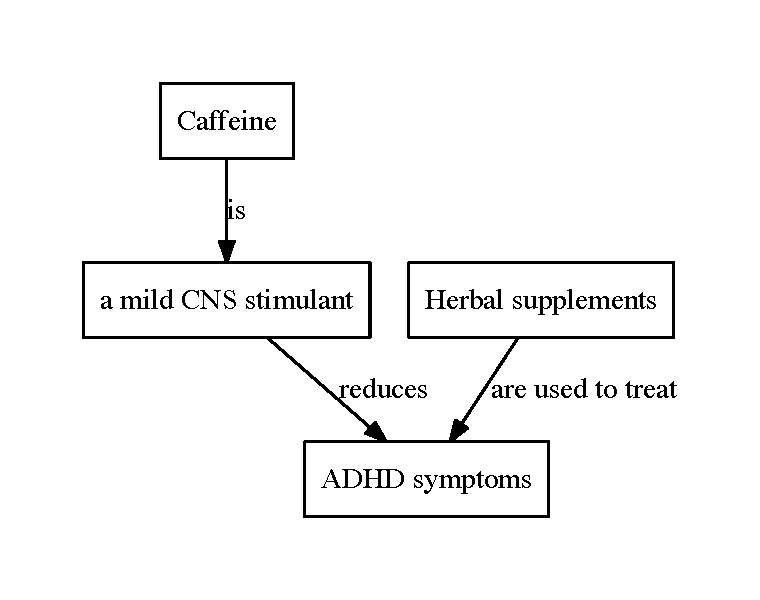
\includegraphics[width=0.5\linewidth]{assets/figures/concept_map}
\caption{Example of a concept map}
\label{fig:concept_map}
\end{figure}
\todo{"Capture important concepts and the structure of texts (spanning over whole text)"}
\todo{Creation of concept maps via library by Tobias}

\paragraph{Co-Occurrence Graph}
\todo{Window size}

\subsubsection{Graph Kernel}
\todo{Categories of graph kernels, eg. random-walk-based, subtree-based}
